\documentclass[a4paper,14pt]{article} 


\usepackage{fontenc}			
\usepackage[utf8]{inputenc}			
\usepackage[english,russian]{babel}	

\usepackage{graphicx, scalerel}    
\usepackage{wrapfig}               
\usepackage[14pt]{extsizes}        
\usepackage[warn]{mathtext}       
\usepackage{indentfirst}      
\usepackage{geometry}
\usepackage[table,xcdraw]{xcolor} 
\usepackage{amsmath,amsfonts,amssymb,amsthm,mathtools}
\usepackage{wasysym}                
\usepackage{upgreek}                
\usepackage{caption}
\usepackage{multirow}
\captionsetup{labelsep=period}
\usepackage[font=small,labelfont=bf]{caption}
\usepackage{gensymb}
\usepackage[unicode, pdftex]{hyperref}
\usepackage{fancyhdr}
\setlength\fboxsep{3pt}
\setlength\fboxrule{1pt}
\usepackage{tocloft}
\usepackage[pdftex]{lscape}
\usepackage{icomma}
\setlength{\arrayrulewidth}{0.4mm}
\usepackage{setspace}
\usepackage{pdfpages}
\usepackage{cmap}

\graphicspath{pictures/}


\newcommand{\tocsection}[1]{\section*{#1} \addcontentsline{toc}{section}{#1}}
\newcommand{\tocsubsection}[1]{\subsection*{#1} \addcontentsline{toc}{subsection}{#1}}
\renewcommand{\cftsecleader}{\cftdotfill{\cftdotsep}}

\newcommand{\comment}[1]{}


\geometry{a4paper,
		  total={170mm,257mm},
		  left=30mm,
		  right=15mm,
		  top=20mm,
		  bottom=20mm}
\onehalfspacing
\setlength{\parindent}{12.5mm}

\bibliographystyle{plain}


\begin{document}
	\newcommand{\HRule}{\rule{\linewidth}{0.7mm}}

\begin{center}
	\large\textbf{Московский Физико-Технический Институт}\\
	\vfill
		
	\Large Микроархитектура современных микропроцессоров
	\\[0.4cm]
	{ \huge \bfseries Replacement Policies}
	\\[0.4cm]
	
	\ \\
	\textbf{\large Автор:} \\	
	\large Овсянников Михаил\\
	\vfill
	\large Долгопрудный, 2025
\end{center}

\thispagestyle{empty}

\newpage
\setcounter{page}{2}

	\newpage
	
	\tableofcontents
	\newpage
	
	\tocsection{Introduction}
	\tocsubsection{Question 1}

	\textit{Приведите формулы для Performance, Power / Dynamic Power, назовите параметры в них входящие}

	\tocsubsection{Answer 1}
	Формула для Performance:
	\begin{equation*}
		Performace = \frac{1}{Time} = \frac{1}{N_\text{instr} \cdot CPI \cdot T_\text{cycle}} = \frac{1}{N_\text{instr}} \cdot IPC \cdot f
	\end{equation*}
	
	Здесь:
	\begin{itemize}
		\item $N_\text{instr}$ -- количество инструкций
		\item $CPI$ -- cycle per instruction, то есть количество тактов на одну инструкцию
		\item $T_\text{cycle}$ -- время одного такта процессора
		\item $IPC$ -- instruction per cycle, то есть количество инструкций за один такт
		\item $f$ -- частота процессора
	\end{itemize}
	
	Формула для Power:
	\begin{equation*}
		P = C \cdot V^2 \cdot f + P_\text{leakage}
	\end{equation*}
	
	Первая часть являет собой Dynamic Power:
	\begin{equation*}
		P_\text{dyn} = C \cdot V^2 \cdot f
	\end{equation*}
	
	В последних двух формулах:
	\begin{itemize}
		\item $C$ -- общая ёмкость элементов
		\item $V$ -- напряжение
		\item $f$ -- частота
		\item $P_\text{leakage}$ -- мощность утечек элементов
	\end{itemize}
	
	\tocsubsection{Question 2}
	\textit{Объясните законы Мура (Moore’s law) и Деннарда (Dennard scaling)}
	
	\tocsubsection{Answer 2}
	\textbf{Закон Мура:} количество транзисторов, размещаемых на кристалле интегральной схемы, удваивается каждые 2 года.
	
	\textbf{Закон Деннарда:} с каждым поколением технологий размеры транзисторов становятся меньше, но потребляемая мощность на единицу площади на кристалле остаётся одинаковой. Напряжение и ток уменьшаются при уменьшении размеров транзисторов.
	
	\tocsubsection{Question 3}
	\textit{Когда закончился Dennard scaling? Чем знаменуется его окончание?}
	
	\tocsubsection{Answer 3}
	Dennard Scaling перестал соблюдаться около 2006 года, поскольку мощность утечек не масштабируется с размером транзисторов. Его окончание повлекло за собой смену тренда -- производители процессоров стали фокусироваться на многоядерных процессорах для улучшения производительности.
	
	\tocsubsection{Question 4}
	\textit{В чем заключается идея Bypassing / Data forwarding оптимизации?}
	
	\tocsubsection{Answer 4}
	Опишем идею bypassing/data forwarding. При конвейерном исполнении инструкций в процессоре могут быть некоторые зависимости по данным или результатам исполнения одной инструкции от другой. Причём, обе эти инструкции могут исполняться одновременно в процессоре, но на разных стадиях конвейера. Без оптимизации придётся ждать, пока данные от ранней инструкции будут записаны по назначенному месту (destination -- register or memory) для того, чтобы исполнить позднюю инструкцию. То есть, несколько тактов процессор будет простаивать, что нехорошо для производительности. При использовании bypassing/data forwarding есть провода, соединяющие разные стадии конвейера, чтобы напрямую получить результат операции, а не ждать, пока он будет записан в регистр/память.
	\begin{figure}[h!]
		\centering
		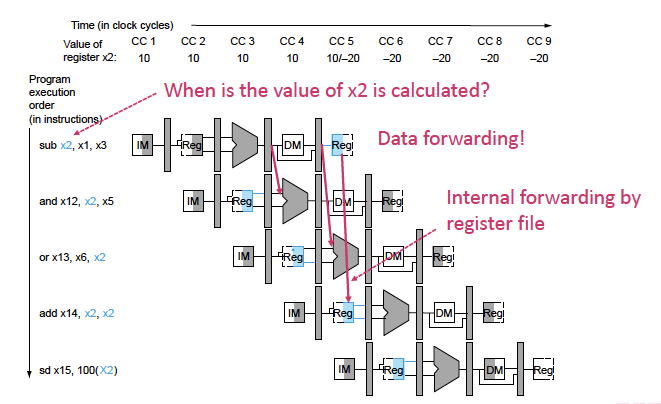
\includegraphics[width=\linewidth]{pictures/bypassing.png}
		\caption{Bypassing}
	\end{figure}
	
	\tocsubsection{Question 5}
	\textit{Что такое Instruction-Level Parallelism? Приведите примеры оптимизаций для его повышения}
	
	\tocsubsection{Answer 5}
	Instruction-Level Parallelism -- это процесс одновременного исполнения нескольких инструкций на процессоре. То есть, в один и тот же такт исполняются сразу несколько инструкций. Конвейер процессора -- это один из примеров Instruction-Level Parallelism, поскольку в один такт исполняются сразу несколько инструкций, хоть они все и на разных стадиях конвейера.
	
	Примеры оптимизаций для повышения Instruction-Level Parallelism:
	\begin{itemize}
		\item Суперскалярность процессора
		\item VLIW архитектура (Very Long Instruction Word architecture)
		\item Векторные CPU, поддержка векторных инструкций
	\end{itemize}
	
	\newpage
	\tocsection{Out-of-Order}
	
	\tocsubsection{Question 1}
	\textit{Для чего нужен Reorder Buffer (ROB)?}
	
	\tocsubsection{Answer 1}
	В Out-of-Order процессоре инструкции записываются в порядке следования в ROB. Эти инструкции исполняются и в итоге покидают ROB. Но каждая инструкция покидает ROB и обновляет архитектурное состояние процессора только если она самая старая в нём и была исполнена. Таким образом, ROB является некоторым хранилищем инструкций, каждая из которых покидает его только если она и все инструкции до неё были исполнены. Создаётся видимость In-Order исполнения, хотя инструкции, находящиеся внутри ROB, могли исполняться в произвольном порядке. Это позволяет достичь большей производительности.
	
	\tocsubsection{Question 2}
	\textit{В чем сложность сделать ROB размером 10000 ячеек даже в случае доступной площади и power ресурса?}
	
	\tocsubsection{Answer 2}
	Существует несколько ограничений, не позволяющих делать (или делающих бесполезным) ROB крайне большого размера:
	\begin{itemize}
		\item Зависимости инструкций: WAR и WAW зависимости крайне неприятны при Out-of-Order исполнении
		\item Исключения: исключения аппаратуры должны происходить только в том порядке и тех местах, как если бы инструкции исполнялись In-Order
		\item Ветвления потока управления: при встрече инструкции, влияющей на поток исполнения, процессору необходимо предугадать, по какой ветви пойдёт исполнение и уже основываясь на этом загружать инструкции в ROB. Если окажется, что предсказание было ложным, то все выполненные инструкции по неверной ветви придётся очистить (flush). Таким образом, теряется производительность
	\end{itemize}
	
	\tocsubsection{Question 3}
	\textit{Как бороться с False/Anti-Dependencies по регистрам? Что такое Register Alias Table?}
	
	\tocsubsection{Answer 3}
	Для борьбы с False/Anti-Dependencies аппаратура может содержать больше регистров в спекулятивном состоянии, чем количество архитектурных регистров, и во время исполнения инструкций производить динамический Register Renaming (количество архитектурных регистров не меняется).
	
	\textbf{Register Alias Table} -- это таблица, в которой хранится соответствие архитектурных и аппаратурных регистров.
	
	\tocsubsection{Question 4}
	\textit{Для чего нужна Instruction Queue (IQ) (по другому Scheduler Queue (SQ) или Reservation Station)? Когда инструкции удаляются из ROB, а когда из Scheduler Queue?}
	
	\tocsubsection{Answer 4}
	Instruction Queue необходима для хранения ещё не исполненных инструкций. Размер IQ значительно меньше размера ROB, что увеличивает производительность, поскольку поиск готовых исполниться инструкций ускоряется (вместо поиска по всему ROB достаточно произвести поиск лишь в IQ). В отличие от ROB, в Instruction Queue хранятся только ещё не исполненные инструкции.
	
	Инструкция удаляется из ROB только тогда, когда она и все предшествующие были исполнены.
	
	Инструкция удаляется из IQ только тогда, когда она была исполнена.
	
	\tocsubsection{Question 5}
	\textit{Что такое Memory Disambiguation проблема? Как с ней бороться?}
	
	\tocsubsection{Answer 5}
	Memory Disambiguation -- это проблема исполнения инструкций доступа в память в Out-of-Order исполнении. Для борьбы с этой проблемой существует набор правил, который помогает при исполнении Store и Load инструкций.
	
	Для Store инструкций:
	\begin{itemize}
		\item Никогда не исполняются спекулятивно, поскольку произвести откат для данной инструкции невозможно или очень сложно
		\item Всегда исполняются в том порядке, в каком идут в коде программы (не перемешиваются между собой)
	\end{itemize}
	
	Для Load инструкций:
	\begin{itemize}
		\item Необходимо дождаться, пока все предшествующие Store инструкции были исполнены (или, если иметь дело только с истинными зависимостями, дождаться, пока один конкретный Store будет исполнен)
	\end{itemize}
	
	Для дальнейших улучшений используются:
	\begin{itemize}
		\item Проверка на пересечение по адресу для инструкций Store/Load
		\item Store Forwarding
		\item Store Buffer и Load Buffer
		\item Разбитие Store инструкции на операции вычисления адреса и вычисления данных
		\item Спекулятивное исполнение Load инструкций
	\end{itemize}
	
	\tocsubsection{Question 6}
	\textit{Объясните смысл разделения Store инструкции на Store Address/Store Data микрооперации}
	
	\tocsubsection{Answer 6}
	Для проверки пересечения инструкций Store и Load значение данных не нужно. Адрес в памяти вычисляется, когда операция Store исполняется. Однако инструкция Store отправляется на исполнение только тогда, когда все её входные параметры (адрес и данные) уже готовы. Отсюда вытекает мнимая зависимость от данных (от которых на самом деле нет зависимости).

	Для избежания такого рода проблем Store делится на две микрооперации:
	\begin{itemize}
		\item STA -- вычисление адреса записи в память
		\item STD -- вычисление данных для записи в память
	\end{itemize}
	
	В этом случае инструкция Load должна ожидать исполнения STD только тогда, когда есть пересечение с соответствующей микрооперацией STA.
	
	\tocsubsection{Question 7}
	\textit{Что такое Load speculation оптимизация?}
	
	\tocsubsection{Answer 7}
	Разбиение инструкции Store на две микрооперации STA и STD действительно ускоряет процесс исполнения, но можно добиться ещё лучших результатов. Можно исполнять инструкции Load спекулятивно, не дожидаясь исполнения STA, а потом, после исполнения STA, проверить результат на корректность.
	
	
	\newpage
	\tocsection{Branch Prediction}

	\tocsubsection{Question 1}
	\textit{Какую информацию хранит Branch Target Buffer?}

	\tocsubsection{Answer 1}
	Branch Target Buffer используется для предсказания адреса перехода для инструкций перехода.
	
	По сути -- это кэш, хранящий для каждой встреченной инструкции перехода предсказание для её адреса перехода.

	\tocsubsection{Question 2}
	\textit{Опишите, как вы бы представили state-of-the-art предсказатель условных переходов на данный момент}
	
	\tocsubsection{Answer 2}
	Я бы представил state-of-the-art предсказатель условных переходов на данный момент как чисто PPM-like предсказатель или как гибрид PPM-like и предсказателей, основанных на модели перцептрона. Для меня яркий пример state-of-the-art предсказателя условных переходов на данный момент -- это TAGE.
	
	\begin{figure}[h!]
		\centering
		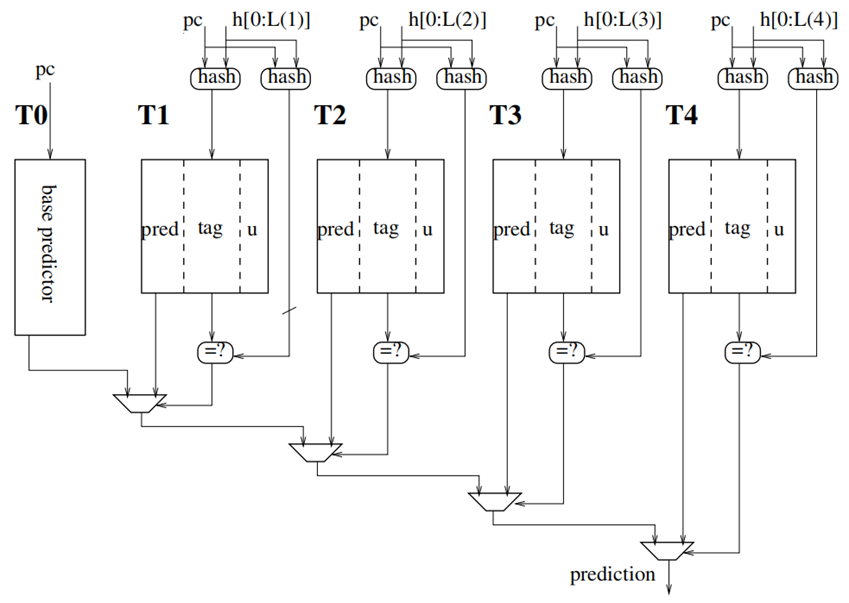
\includegraphics[width=\linewidth]{pictures/TAGE.png}
		\caption{TAGE предсказатель переходов}
	\end{figure}
	
	TAGE -- это TAgged GEometric history length. Во внимание принимается не только самая длинная последовательность, но и вторая по длине тоже. Небольшой метапредсказатель делает окончательное предсказание на основе всего состояния TAGE. Это сделано для решения проблемы холодного счётчика.
	
	\tocsubsection{Question 3}
	\textit{Процессор имеет двухуровневый адаптивный предсказатель условных переходов (two-level adaptive conditional branch predictor). Предсказатель хранит направления последних бранчей (branch direction) из глобальной истории (global history) в регистре истории (BHR) размером 3 бита. Pattern History Table имеет размер 8 и использует стандартные 2-битные счетчики с насыщением (2-bit saturating counters). В начальных момент времени счетчики находятся в состоянии “Strongly Not Taken”. Рассчитайте misprediction rate (процент неверных предсказаний) для данного предсказателя условных переходов в случае исполнения программы ниже}
	
	\newpage
 	\begin{minted}{cpp}
#include <iostream>
		
int main() {
    for (int i = 0; i < 100; ++i) {
        std::cout << i << "\n";
    }
    return 0;
}
	\end{minted}
	
	\tocsubsection{Answer 3}
	Ответ неоднозначный. Зависит от нескольких факторов, но главный из них -- это компилятор. Реализовать цикл можно двумя разными способами.
	
	Ссылка на Godbolt: \href{https://godbolt.org/z/bnbcbEc7b}{https://godbolt.org/z/bnbcbEc7b}

	Первый вариант (например, Clang):
	\begin{minted}{nasm}
loop_check:
    cmp i, 100
    jge #loop_exit

loop_body:
    ...
    inc i
    jmp #loop_header

loop_exit:
    ...
	\end{minted}

	\newpage
	Второй вариант (например, GCC):
	\begin{minted}{nasm}
loop_header:
    jmp #loop_check

loop_body:
    ...
    inc i

loop_check:
    cmp i, 99
    jle #loop_body
    ...
	\end{minted}
	
	Два варианта кардинально отличаются. Разберём их отдельно.
	
	Положим, что бит 0 в BHR соответствует состоянию Not Taken, а бит 1 -- Taken. Также положим, что начальное состояние BHR -- это три нуля.
	
	\textbf{Вариант 1}

	\begin{figure}[h!]
		\centering
		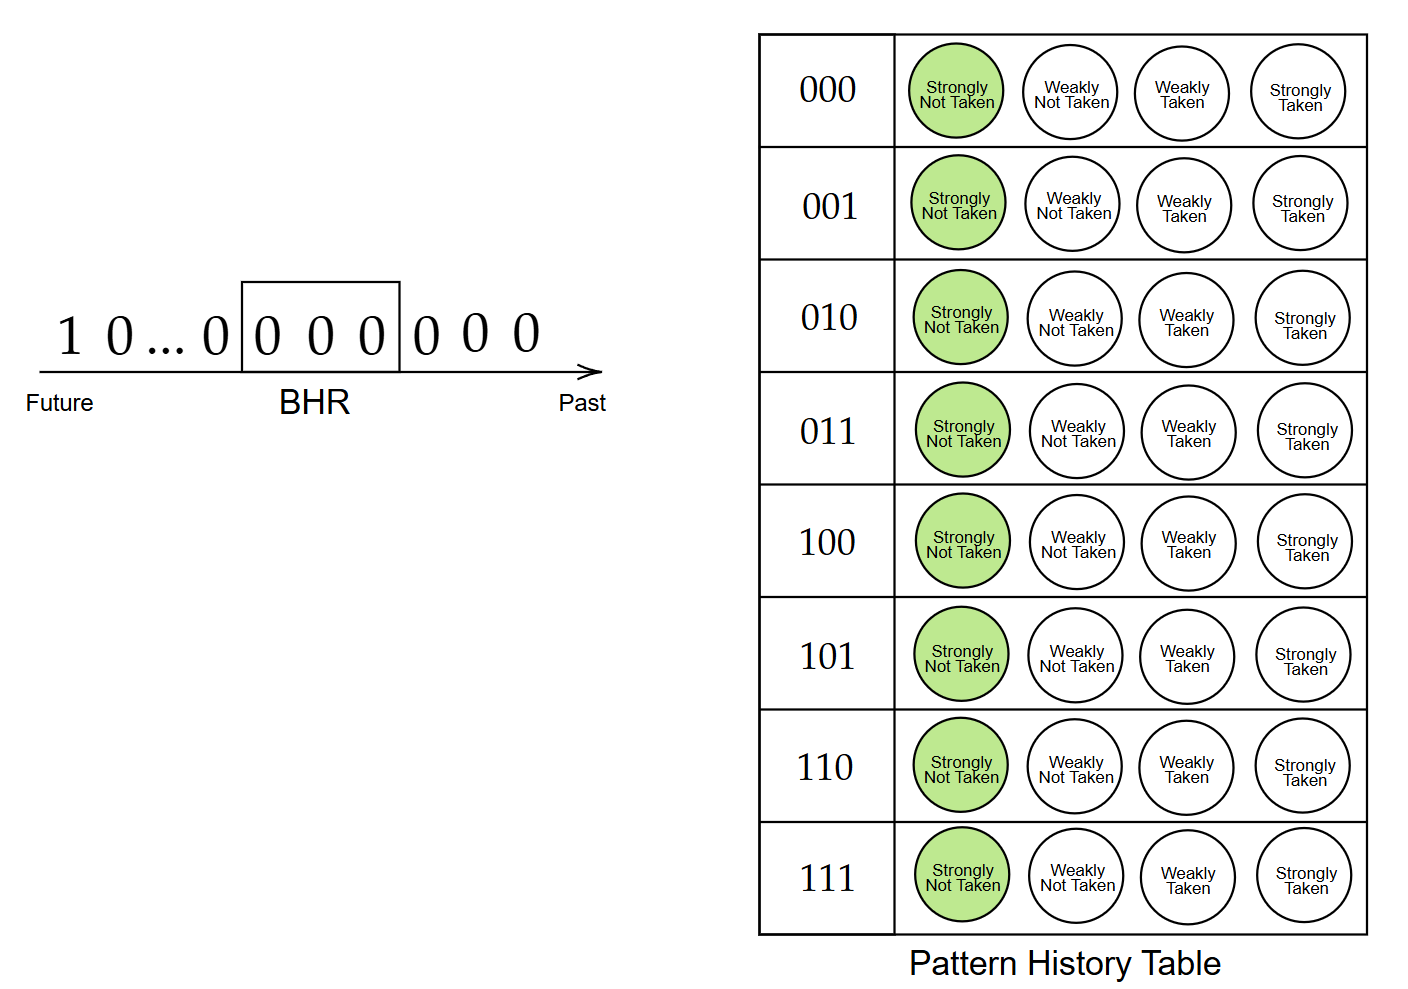
\includegraphics[width=\linewidth]{pictures/BHR_PHT_1.png}
		\caption{Вариант 1}
	\end{figure}

	В первом варианте инструкция перехода исполняется 101 раз: 100 раз Not Taken и 1 раз Taken. Учитывая начальные состояния BHR и PHT, то получается, что с самого начала предсказания будут корректными и лишь самый последний раз, при выходе из цикла, предсказание будет ошибочным -- в BHR будет 000, а все ячейки PHT будут иметь значение Strongly Not Taken, хотя на самом деле переход будет исполнен.
	
	При таком сценарии количество неверных предсказаний -- это 1, а всего их -- 101. Получается:
	\begin{equation*}
		Misprediction = \frac{1}{101} \simeq 0.009901 \hspace*{6pt} (0.9901 \%)
	\end{equation*}

	\newpage
	\textbf{Вариант 2}

	Во втором варианте инструкция перехода исполняется 101 раз: 100 раз Taken и 1 раз Not Taken.
	\begin{itemize}
		\item В первый раз состояние BHR -- 000. Соответствующая ячейка в PHT хранит Strongly Not Taken. Это первое неверное предсказание
		\item Во второй раз состояние BHR -- 100. Соответствующая ячейка в PHT хранит Strongly Not Taken. Это второе неверное предсказание		\item В третий раз состояние BHR -- 110. Соответствующая ячейка в PHT хранит Strongly Not Taken. Это третье неверное предсказание		\item В четвертый раз состояние BHR -- 111. Соответствующая ячейка в PHT хранит Strongly Not Taken. Это четвертое неверное предсказание
		\item В пятый раз состояние BHR снова 111. Соответствующая ячейка в PHT хранит Weakly Not Taken. Это пятое неверное предсказание
		\item Начиная с этого момента, предсказания станут верными, поскольку состояние BHR всегда будет 111, а ячейка PHT -- Taken
		\item ...
		\item В 101-ый раз состояние BHR -- 111. Соответствующая ячейка в PHT хранит Strongly Taken. Это шестое неверное предсказание
	\end{itemize}

	При таком сценарии количество неверных предсказаний -- это 6, а всего их -- 101. Получается:
	\begin{equation*}
		Misprediction = \frac{6}{101} \simeq 0.059406 \hspace*{6pt} (5.9406 \%)
	\end{equation*}
	
	\tocsubsection{Question 4}
	\textit{Объясните связь двухуровневых адаптивных предсказателей (two-level adaptive branch predictor) и алгоритма PPM (Prediction by Partial Matching)}
	
	\tocsubsection{Answer 4}
	\begin{figure}[h!]
		\centering
		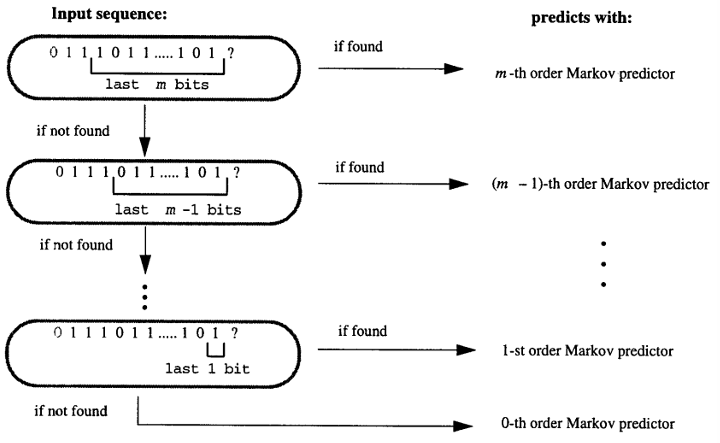
\includegraphics[width=\linewidth]{pictures/PPM.png}
		\caption{Prediction by Partial Matching}
	\end{figure}

	Для наглядности продемонстрируем связь на примере Markov Predictor порядка $m$.

	\begin{figure}[h!]
		\centering
		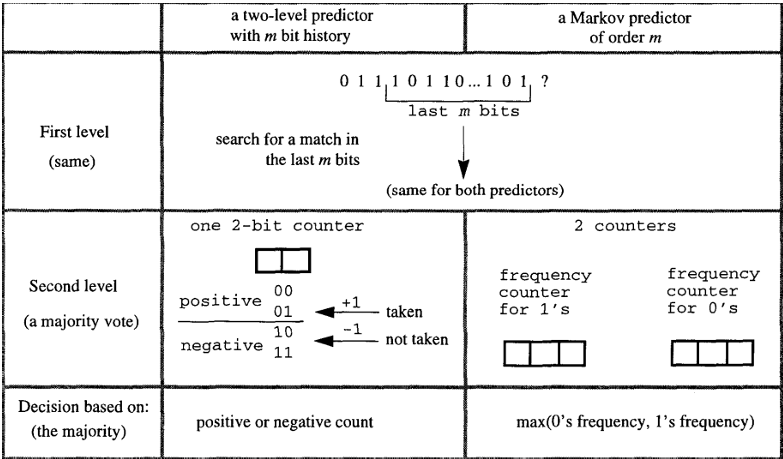
\includegraphics[width=\linewidth]{pictures/two-level-vs-ppm.png}
		\caption{Two-level adaptive branch predictor vs PPM}
	\end{figure}
	
	Оба алгоритма рассматривают последние $m$ бит входной последовательности. Но в двухуровневых адаптивных предсказателях для каждой такой подпоследовательности используются 2-битные счётчики с насыщением, а у Markov Predictor -- обыкновенные счётчики частоты появления. Окончательное предсказание делается тоже по-разному: в двухуровневых адаптивных предсказателях -- по положительному/отрицательному значению счётчика (то есть к какой его границе ближе); а в Markov Predictor -- выбирается на основе максимальной частоты появления.
	
	Оба алгоритма хорошо динамически подстраиваются под поведение программы для предсказания переходов.
	
	\tocsubsection{Question 5}
	\textit{Какими полезными свойствами обладает перцептрон (perceptron) с точки зрения обработки входных данных? Опишите, какую функцию выполняет перцептрон в случае использования в виде статистического корректора (statistical corrector)}
	
	\tocsubsection{Answer 5}
	Предсказатели на основе модели перцептрона очень хороши при комбинировании входных данных разных типов.
	
	Предсказатель переходов TAGE крайне эффективен при предсказании коррелированных переходов. Однако он плохо предсказывает переходы, которые статистически более связаны с направлением перехода, а не с их историей, или вообще некоррелированны. Для лучших предсказаний таких переходов был предложен Statistical Corrector -- небольшой предсказатель, который нацелен на детектирование маловероятного предсказания от самого TAGE и инвертирование его. Для этого ему необходима информация об инструкции перехода: адрес, глобальная история переходов, глобальный путь управления, локальная история и т.п.
	
	\tocsubsection{Question 6}
	\textit{Какие виды условных переходов являются сложно-предсказываемыми для предсказателя TAGE?}
	
	\tocsubsection{Answer 6}
	Для TAGE слабо коррелированные или совсем некоррелированные переходы (weakly-biased branches) являются сложно-предсказываемыми. Именно поэтому и был предложен Statistical Corrector.
	
	\tocsubsection{Question 7}
	\textit{Объясните основный смысл рассмотренной на лекции статьи ''Branch Prediction is Not a Solved Problem''}
	
	\tocsubsection{Answer 7}
	Несмотря на то, что в мире уже существует огромное множество разных предсказателей переходов, которые дают ощутимый прирост производительности, проблема предсказания переходов остаётся актуальной, потому что по оценкам за оставшимися процентами неверных предсказаний (misprediction rate) скрывается ещё около $20\%$ производительности (IPC). Главные причины этого: существование сложно-предсказываемых переходов и наличие переходов, которые в динамике крайне редко исполняются, поэтому они вносят вклад в misprediction rate.
	
	
	\newpage
	\tocsection{Memory}
	
	\tocsubsection{Question 1}
	\textit{В чем разница между Fully Associative, Direct Mapped и Set-Associative кэшами?}
	
	\tocsubsection{Answer 1}
	\textbf{Fully Associative}:
	\begin{itemize}
		\item Кэш-линии может быть сопоставлена произвольная ячейка кэша. Поэтому поиск происходит по всему кэшу
		\item Адрес разбивается на номер линий (тег) и смещение внутри неё. Поэтому коллизии невозможны
		\item Каждая ячейка кэша имеет тег. Поэтому номер линии адреса сравнивается со всеми ячейками кэша в параллель
	\end{itemize}
	
	\textbf{Direct Mapped}
	\begin{itemize}
		\item Кэш-линии может быть сопоставлена лишь определенная ячейка кэша. Поэтому для поиска необходима только одна ячейка
		\item Адрес разбивается на номер линий (тег), номер ячейки кэша (сет) и смещение внутри неё. Поэтому коллизии возможны
	\end{itemize}


	\textbf{N-Way Set-Associative}
	\begin{itemize}
		\item Кэш-линии может быть сопоставлена лишь определенный набор ячеек кэша (набор ways для каждого сета)
		\item Адрес также разбивается на номер линий (тег), номер ячейки кэша (сет) и смещение внутри неё. Поэтому коллизии возможны, но происходят сильно реже, чем в Direct Mapped кэше
	\end{itemize}
	
	\tocsubsection{Question 2}
	\textit{Для чего используется Translation Lookaside Buffer (TLB)?}
	
	\tocsubsection{Answer 2}
	Для безопасности (и иногда эффективности) программы работают не с физической памятью, а с виртуальной. Процессору необходим настоящий, физический, адрес для операций с памятью. За трансляцию адресов ответственны MMU (Memory Management Unit) и операционная система. Но это достаточно долгий процесс, поэтому существует (Translation Lookaside Buffer) TLB -- это небольшой кэш для транслированных адресов для ускорения этого процесса.
	
	\tocsubsection{Question 3}
	\textit{Что такое гранулярность политик замещения?}
	
	\tocsubsection{Answer 3}
	Гранулярность политик замещения отвечает за то, по каким критериям и на каких стадиях выделять ячейки кэша. Существуют крупные, или крупнозернистые (coarse-grained), и тонкие, или мелкозернистые (fine-grained), политики замещения. В первых кэш-линии различаются лишь на поведении в кэше, а вторые -- ещё вдобавок при вставке в кэш.
	
	\tocsubsection{Question 4}
	\textit{Какие есть стандартные паттерны обращения к кэшу?}
	
	\tocsubsection{Answer 4}
	\begin{figure}[h!]
		\centering
		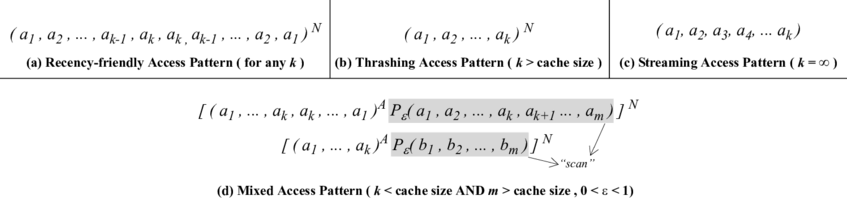
\includegraphics[width=\linewidth]{pictures/access-patterns.png}
		\caption{Стандартные паттерны обращения к кэшу}
	\end{figure}
	
	Паттерны обращения к кэшу:
	\begin{itemize}
		\item Recency-friendly
		\item Thrashing
		\item Streaming
		\item Mixed (Scanning)
	\end{itemize}

	\tocsubsection{Question 5}
	\textit{В каком ключе LRU Insertion Policy (LIP) лучше классической LRU политики замещения?}

	\tocsubsection{Answer 5}
	LRU Insertion политика очень похожа на классическую LRU. Отличие только в том, что при вставке в кэш в LIP выбирается LRU позиция (самая давняя), а классическом LRU -- MRU позиция (самая новая). Благодаря этому LIP более устойчив паттерну обращения Thrashing.
	
	\tocsubsection{Question 6}
	\textit{За счет чего BRRIP политика замещения является устойчивой к scanning и thrashing паттернам?}
	
	\tocsubsection{Answer 6}
	Политика замещения BRRIP устойчива к паттерну обращения к кэшу thrashing ровно по той же причине, что и LIP -- если к недавно вставленной линии не было обращения, то она быстро вытесняется из кэша.
	
	Политика замещения BRRIP устойчива к паттерну обращения к кэшу scanning за счёт того, что вставка новых линий происходит ближе к позиции жертвы (victim), причём, с некоторой вероятностью новоявленная линия будет вставлена не непосредственно на позицию жертвы, а лишь перед ней, что позволит ей задержаться в кэше подольше.
	
	\tocsubsection{Question 7}
	\textit{В чем основная идея политик замещения Hawkeye и Mockingjay?}
	
	\tocsubsection{Answer 7}
	Главная идея политик замещения Hawkeye и Mockingjay заключается в том, что, несмотря на то, что предсказать будущее невозможно, можно применить известный алгоритм Белади (Belady) к доступам в память в прошлом. Таким образом, можно обучить предсказатель для того, чтобы предсказывать будущие доступы в память.
	
	\tocsubsection{Question 8}
	\textit{Объясните принцип работы Spatial Memory Streaming (SMS) префетчера}
	
	\tocsubsection{Answer 8}
	\begin{figure}[h!]
		\centering
		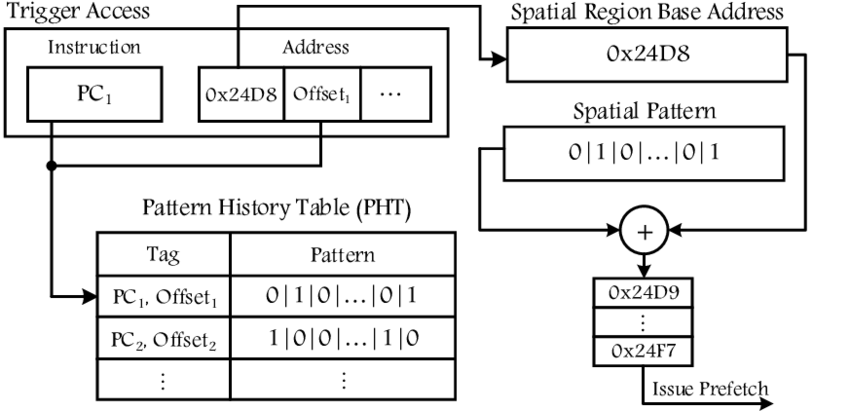
\includegraphics[width=\linewidth]{pictures/SMS.png}
		\caption{Spatial Memory Streaming префетчер}
	\end{figure}
	
	Spatial Memory Streaming (SMS) разделяет адресное пространство на секции фиксированного размера, которые называются Spatial Regions. SMS запоминает паттерны доступа в память в этих секциях, после чего эти паттерны используются для префетчинга будущих доступов в память, если приложение снова обращается к этим или похожим секциям.
	
	\newpage
	\tocsection{Advanced Optimizations \& Parallelism}
	
	\tocsubsection{Question 1}
	\textit{На покрытие какие сложных случаев направлено использование Execution-based Prefetchers?}

	\tocsubsection{Answer 1}
	На покрытие случаев, когда в программе происходит множество обращений в память, которые могут повлечь множество промахов в кэш, из-за чего конвейер процессора будет простаивать (stall).
	
	\tocsubsection{Question 2}
	\textit{Что такое Value Prediction оптимизация? Для каких инструкций, как правило, используется данная оптимизация в современных процессорах?}
	
	\tocsubsection{Answer 2}
	Value Prediction оптимизация заключается в предугадывании результатов инструкций до их непосредственного исполнения. Оптимизация направлена на устранение зависимости по данным и увеличения Instruction-Level Parallelism.
	
	Данная оптимизация, как правило используется для:
	\begin{itemize}
		\item Арифметических инструкций
		\item Load инструкций
		\item Инструкций, которые могут дать ощутимый прирост при малой стоимости ошибки, если вероятность предсказания мала
		\item Инструкций, которые могут дать малый прирост при ощутимой стоимости ошибки, если вероятность предсказания велика
	\end{itemize}
	
	\tocsubsection{Question 3}
	\textit{За счет чего получается прирост производительности в случае применения Value Prediction оптимизации?}
	
	\tocsubsection{Answer 3}
	За счёт устранения некоторых зависимостей по данным и за счёт наличия Value Locality.
	
	\tocsubsection{Question 4}
	\textit{В чем разница между Value Prediction и Branch Prediction с точки зрения необходимости/ожидаемого положительного эффекта от предсказания и последующего спекулятивного исполнения в случае низкой уверенности в точности предсказания?}

	\tocsubsection{Answer 4}
	Оптимизация Branch Prediction предсказывает поток управления программы, а Value Prediction -- непосредственно значения инструкций, что гораздо сложнее. Стоимость ошибки предсказания Branch Prediction мала по сравнению с потенциальным выигрышем при успехе, поэтому данная оптимизация может исполняться спекулятивно всегда. Value Prediction -- напротив -- имеет высокую стоимость ошибки предсказания, но также и более крупный выигрыш при успехе, поэтому для данной оптимизации необходима хорошая уверенность в точности предсказания.
	
	\tocsubsection{Question 5}
	\textit{Что такое Memory Renaming оптимизация?}
	
	\tocsubsection{Answer 5}
	\begin{figure}[h!]
		\centering
		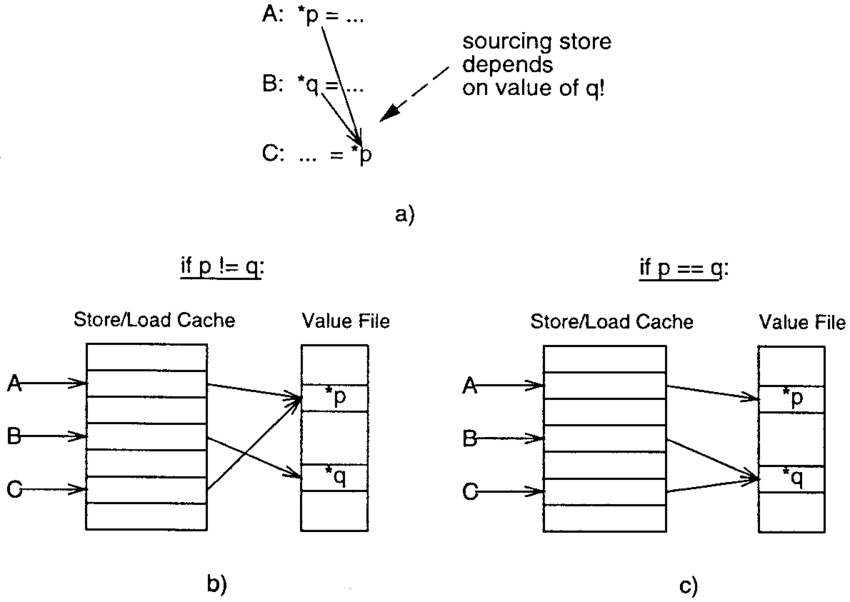
\includegraphics[width=\linewidth]{pictures/memory-renaming.png}
		\caption{Memory Renaming оптимизация}
	\end{figure}

	Memory Renaming -- это оптимизация, направленная на улучшение коммуникации инструкций load/store с памятью, которая находит, кэширует и использует зависимости между load/store инструкциями. Как только определенная зависимость между load/store инструкциями была найдена, записи в память с помощью инструкции store могут быть перенаправлены напрямую к зависимым от них инструкциям load. Таким образом, улучшается коммуникация инструкций load/store с памятью и, следовательно, производительность.

	Оптимизация вносит некоторые дополнительные правила работы с инструкциями load/store.
	
	Для инструкции Store:
	\begin{minted}{cpp}
if (not in store/load cache) {
    allocate store/load cache entry for store
    allocate value file entry for store result
    point store/load cache entry to value file entry
}
deposit store result into value file and memory
	\end{minted}
	
	Для инструкции Load:
	\begin{minted}{cpp}
if (not in store/load cache) {
    allocate store/load cache entry for load
    point store/load cache entry to value file entry of source store
    if no sourcing store, insert result of load into value file
}
return value file entry as load result
	\end{minted}
	
	\tocsubsection{Question 6}
	\textit{Объясните разницу между Fine-Grained Multithreading, Coarse-Grained\\ Multithreading и Simultaneous Multithreading}
	
	\tocsubsection{Answer 6}
	\textbf{Fine-Grained Multithreading}: смена потока на каждом такте процессора -- в конвейере нет двух или более инструкций с одного и того же потока.
	
	\textbf{Coarse-Grained Multithreading}: смена потока при каком-то определенном событии, например, промахе в кэш, синхронизации или по истечении кванта времени.
	
	\textbf{Simultaneous Multithreading}: исполнение инструкций сразу с нескольких потоков в один и тот же такт процессора для большей загрузки его элементов.
	
	\textbf{Fine-Grained Multithreading}:
	\begin{itemize}
		\item Нет нужды для проверки зависимостей между инструкциями
		\item Нет нужды в логике предсказателя переходов (branch predictor)
		\item Пузыри-такты (bubble cycles) используются другими потоками для исполнения инструкций
		\item Улучшенные Throughput, Latency Tolerance и Utilization
		\item Дополнительная сложная логика в аппаратуре
		\item Хуже производительность одного конкретного потока
		\item Борьба потоков за ресурсы памяти и кэша
		\item Всё ещё необходимы проверки логики исполнения между потоками
	\end{itemize}
	
	\textbf{Coarse-Grained Multithreading}:
	\begin{itemize}
		\item Улучшенная производительность одного конкретного потока
		\item Сложнее логика в аппаратуре
		\item Б\'{о}льшая нагрузка при смене контекста
		\item Fairness vs. Throughput проблема
	\end{itemize}
	

	\textbf{Simultaneous Multithreading}:
	\begin{itemize}
		\item Б\'{о}льшая загрузка элементов процессора
		\item Суперскалярные и Out-of-Order процессоры уже имеют поддержку нескольких функциональных устройств
		\item Лучший Throughput
	\end{itemize}
	
	\newpage
	\thispagestyle{empty}
	\vspace*{\fill}
	\begingroup
	\centering
	{\Huge Thank you!}

	\endgroup
	\vspace*{\fill}

\end{document}